\documentclass[tikz,border=2pt]{standalone}

\usepackage{pgfplots}
\pgfplotsset{compat=1.18}

\begin{document}
	
	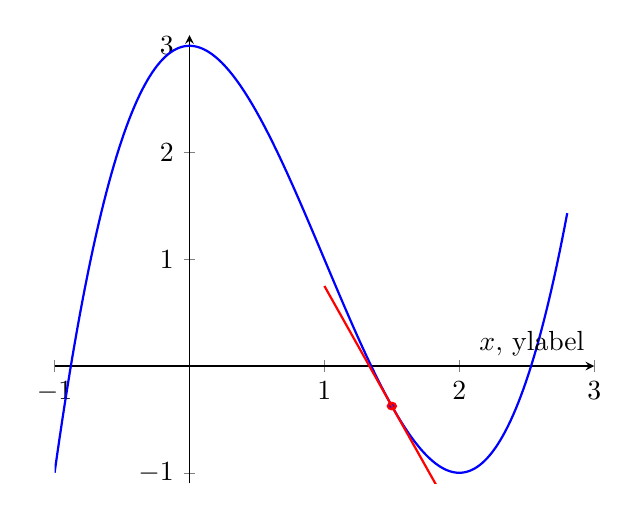
\begin{tikzpicture}
		\begin{axis}[
			axis lines = middle,
			xmin=-1, xmax=3,
			ymin=-1.1, ymax=3.1,
			xlabel = $x\text{,}$
			ylabel = {$y$},
			]
			
			\addplot [thick,
			domain=-1:2.8,
			samples=200,
			color=blue,
			]
			{x*x*x-3*x*x+3};
			\draw [red, thick, fill=blue] (1.5,-0.375) circle [radius=0.03];
			\addplot [thick,
			domain=1:2,
			samples=200,
			color=red,
			]
			{-2.25*x+3};	
		\end{axis}
	\end{tikzpicture}
	
\end{document}